\FloatBarrier

\section{Synthetic and real-data MLP experiments}
\label{sec:mlp}

\subsection{Synthetic MLP}
\label{sec:mlp-synthetic}

The RFNN microscope predicts that widening the latent space adds
low-variance buffer modes before sample-specific modes can be fit.
We next test the same mechanism in a trainable score network. The
synthetic MLP uses the same Gaussian-mixture data as the RFNN
experiment, but the first layer is learned and the score is trained
over diffusion times. To avoid the most obvious confound, we hold
the hidden width fixed across the $\dlat$ sweep; increasing
$\dlat$ therefore changes the latent buffer and output dimension,
but not the hidden-layer capacity.

\begin{figure}[!t]
  \centering
  
\includegraphics[width=0.88\linewidth]{figures/synthetic_mlp_final_mem_ratio.pdf}
  \caption{\textbf{Synthetic MLP memorization decreases with latent
    buffer width.} Five-seed mean final memorization ratio after
    5M steps for a fixed-width MLP, sweeping $\dlat$ at
    $\dint=5$. Memorization falls from roughly $30\%$ at
    $\dlat=5$ to near zero by $\dlat=40$.}
  \label{fig:synthetic-mlp-final-mem}
\end{figure}

\begin{figure}[!t]
  \centering
  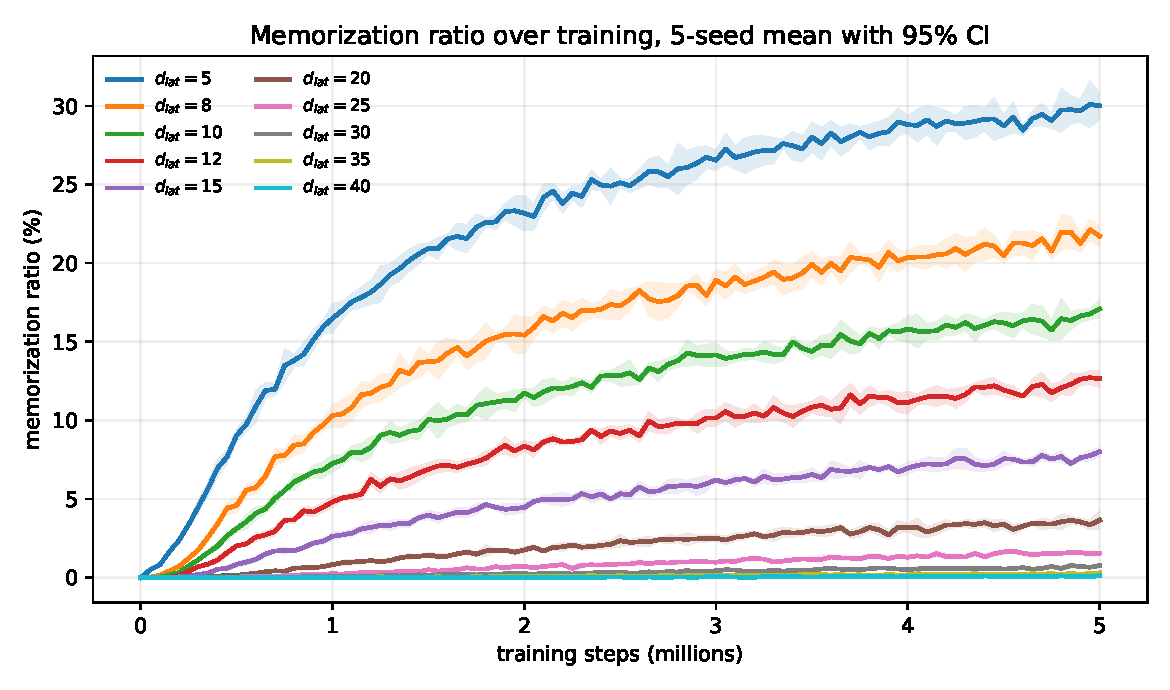
\includegraphics[width=\linewidth]{figures/synthetic_mlp_mem_over_steps.pdf}
  \caption{\textbf{Synthetic memorization trajectories.} The
    same five-seed sweep over training steps. Larger latent spaces
    delay and suppress the onset of memorization under the
    Bonnaire/Somepalli nearest-neighbor ratio test.}
  \label{fig:synthetic-mlp-mem-curves}
\end{figure}

\begin{figure}[!t]
  \centering
  
\includegraphics[width=\linewidth]{figures/synthetic_mlp_score_error_per_dim.pdf}
  \caption{\textbf{Synthetic score error per latent dimension.}
    Normalizing score error by $\dlat$ separates the memorization
    trend from the trivial increase in output dimension. The
    fixed-width MLP remains comparable across the sweep while
    memorization drops sharply.}
  \label{fig:synthetic-mlp-score-error}
\end{figure}

The MLP result is qualitatively sharper than the frozen-feature
prediction: at high $\dlat$, feature learning appears to find
sparser, signal-aligned directions instead of spending equal effort
on all random-feature modes. Nevertheless, the direction of the
effect agrees with the buffer picture: widening the latent space
does not accelerate memorization, and under fixed hidden width it
strongly suppresses it.

\FloatBarrier
\subsection{CelebA and CIFAR-10}
\label{sec:real-data}

Real image latents introduce a second effect absent from the
synthetic construction: if the VAE bottleneck is too narrow, the
training images cannot be reconstructed faithfully, so pixel-space
memorization is hard to detect. We therefore expect a non-monotone
curve. As $\dlat$ first increases, the VAE becomes expressive
enough for the diffusion model to reproduce the 1k-image training
subset; once the latent code is sufficiently expressive, further
increasing $\dlat$ creates an excess-dimensional buffer and
memorization decreases.

\begin{figure*}[!t]
  \centering
  \begin{subfigure}{0.24\textwidth}
    \centering
    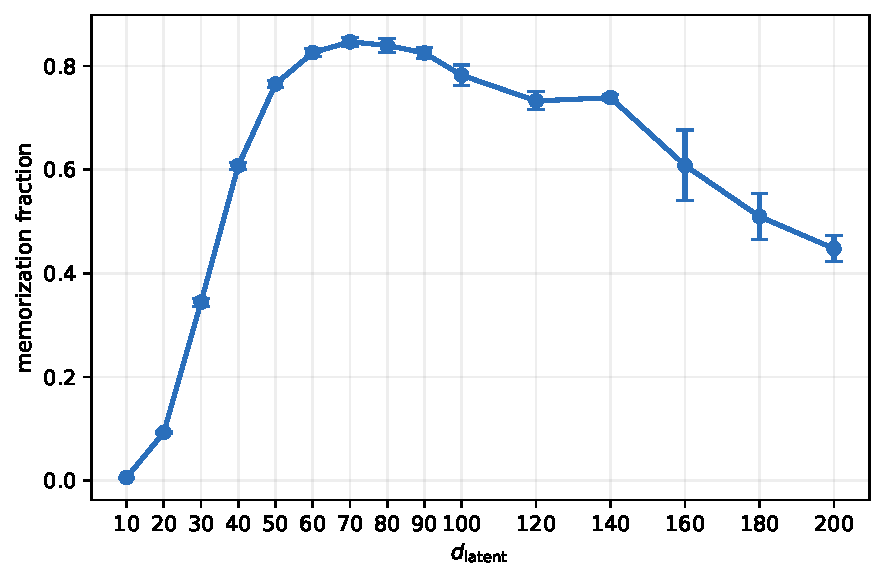
\includegraphics[width=\linewidth]{figures/celeba_final_mem_vs_d.pdf}
    \caption{CelebA mem.}
  \end{subfigure}\hfill
  \begin{subfigure}{0.24\textwidth}
    \centering
    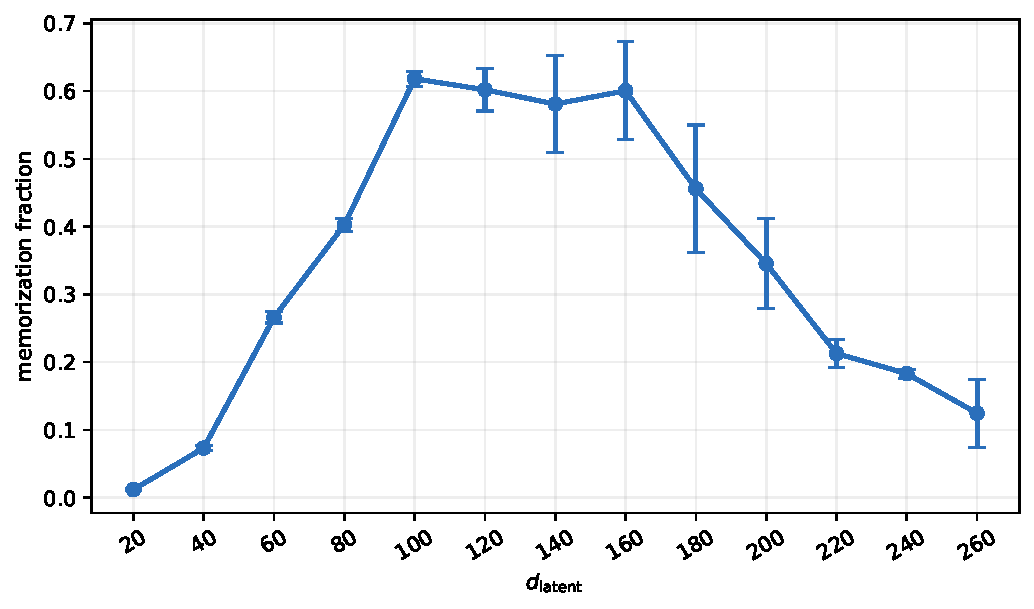
\includegraphics[width=\linewidth]{figures/cifar10_final_mem_vs_d.pdf}
    \caption{CIFAR-10 mem.}
  \end{subfigure}\hfill
  \begin{subfigure}{0.24\textwidth}
    \centering
    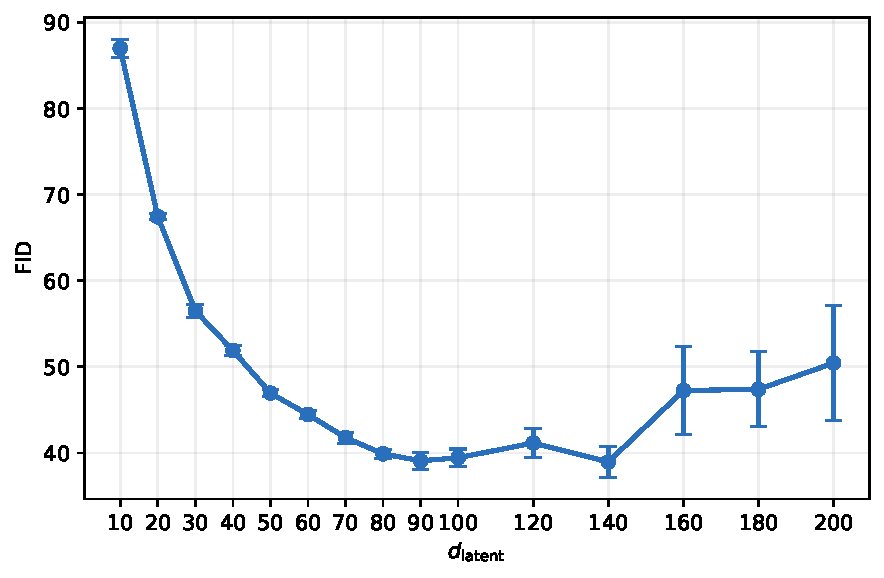
\includegraphics[width=\linewidth]{figures/celeba_final_fid_vs_d.pdf}
    \caption{CelebA FID.}
  \end{subfigure}\hfill
  \begin{subfigure}{0.24\textwidth}
    \centering
    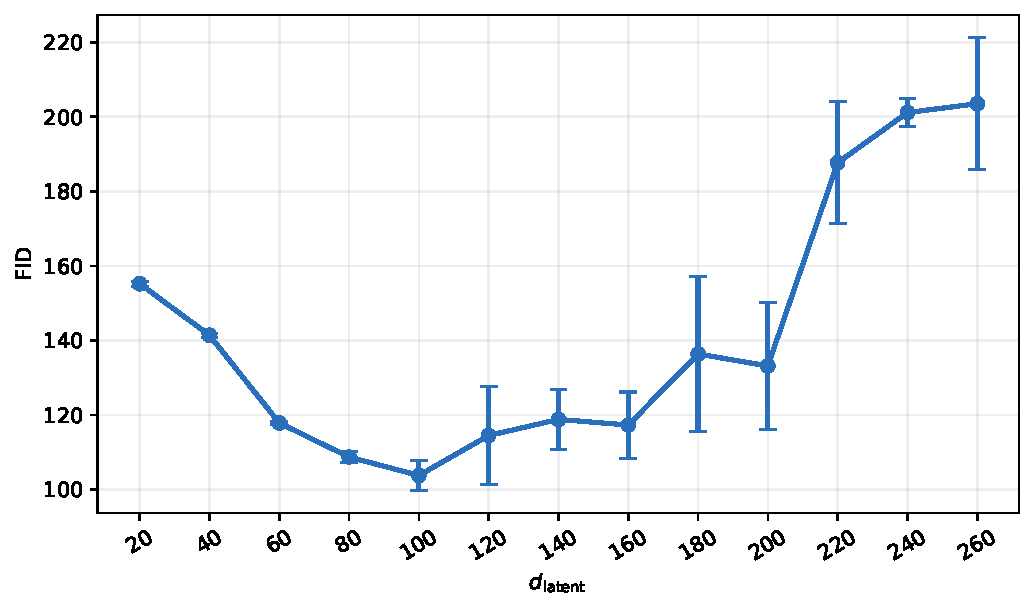
\includegraphics[width=\linewidth]{figures/cifar10_final_fid_vs_d.pdf}
    \caption{CIFAR-10 FID.}
  \end{subfigure}
  \caption{\textbf{Real-data latent width produces a quality--memory
    tradeoff.} Five-seed means with 95\% confidence intervals after
    5M MLP diffusion steps on a diverse 1k subset. On both datasets,
    memorization rises at small-to-moderate $\dlat$ as the VAE
    becomes more faithful, then decreases at larger $\dlat$. FID is
    best at intermediate latent widths and worsens again once the
    latent space is very wide.}
  \label{fig:real-final-mem-fid}
\end{figure*}

On CelebA, final memorization peaks near $\dlat=70$--$80$ and then
falls by roughly half by $\dlat=200$. On CIFAR-10, the peak occurs
near $\dlat=100$ and falls to about $12\%$ by $\dlat=260$. FID
shows the corresponding reconstruction/generation tradeoff:
moderate dimensions improve quality, while very high dimensions
make training harder and degrade FID.

\begin{figure*}[!t]
  \centering
  \begin{subfigure}{0.49\textwidth}
    \centering
    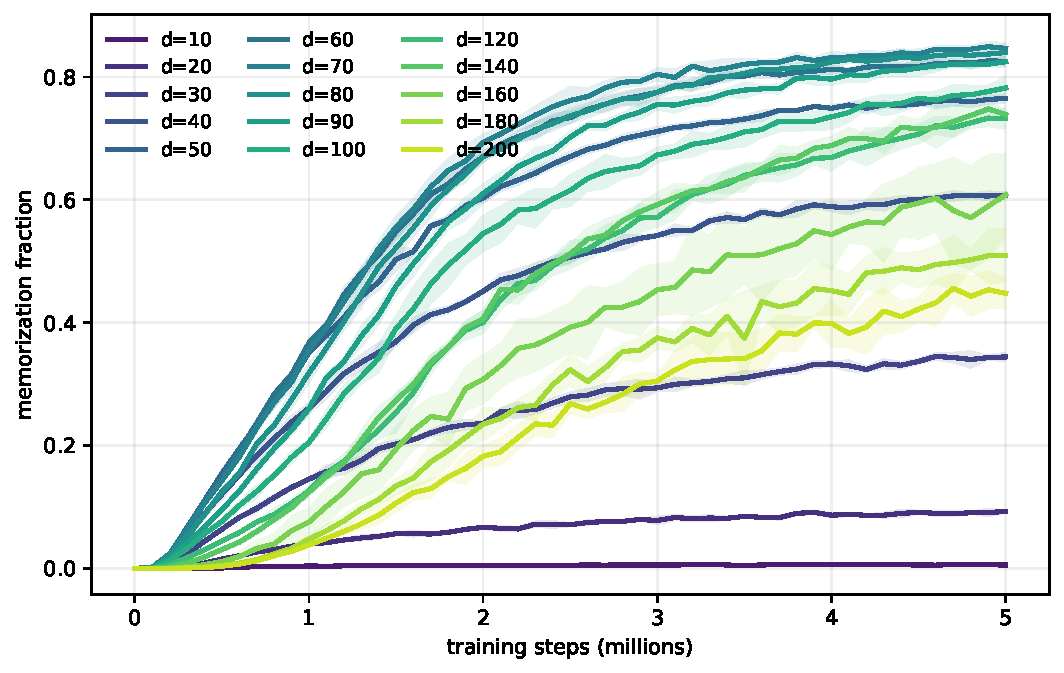
\includegraphics[width=\linewidth]{figures/celeba_mem_over_steps_ci.pdf}
    \caption{CelebA memorization.}
  \end{subfigure}\hfill
  \begin{subfigure}{0.49\textwidth}
    \centering
    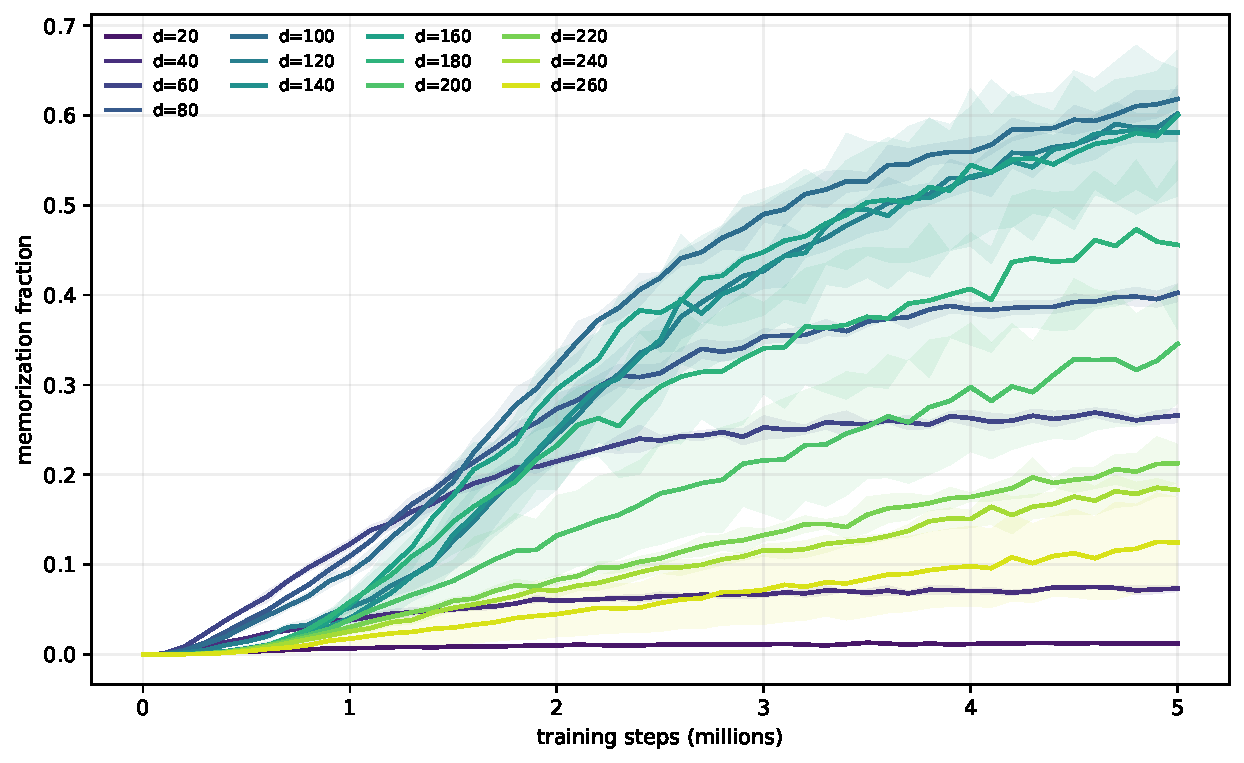
\includegraphics[width=\linewidth]{figures/cifar10_mem_over_steps_ci.pdf}
    \caption{CIFAR-10 memorization.}
  \end{subfigure}
  \caption{\textbf{Memorization over training.} Mean memorization
    fraction over five seeds. High-dimensional CelebA and CIFAR-10
    runs remain below the mid-dimensional peak throughout training,
    rather than merely reaching the same endpoint later.}
  \label{fig:real-mem-curves}
\end{figure*}

\subsection{Data-spectrum predictor}
\label{sec:spectral-predictor}

Finally, we test whether the empirical memorization curves are
predictable from the data geometry alone. For each trained VAE we
encode the same diverse 1k subset, form the diffused latent
covariance spectrum, and compute a spectral pressure curve
$P_d(s)$ that accumulates learned eigenmodes over training step
$s$. A single global calibration maps pressure levels to
memorization thresholds. This is not yet the closed-form theorem;
it is a data-spectrum surrogate that asks whether the geometry of
the latent code contains the right temporal ordering.

\begin{figure*}[!t]
  \centering
  \begin{subfigure}{0.49\textwidth}
    \centering
    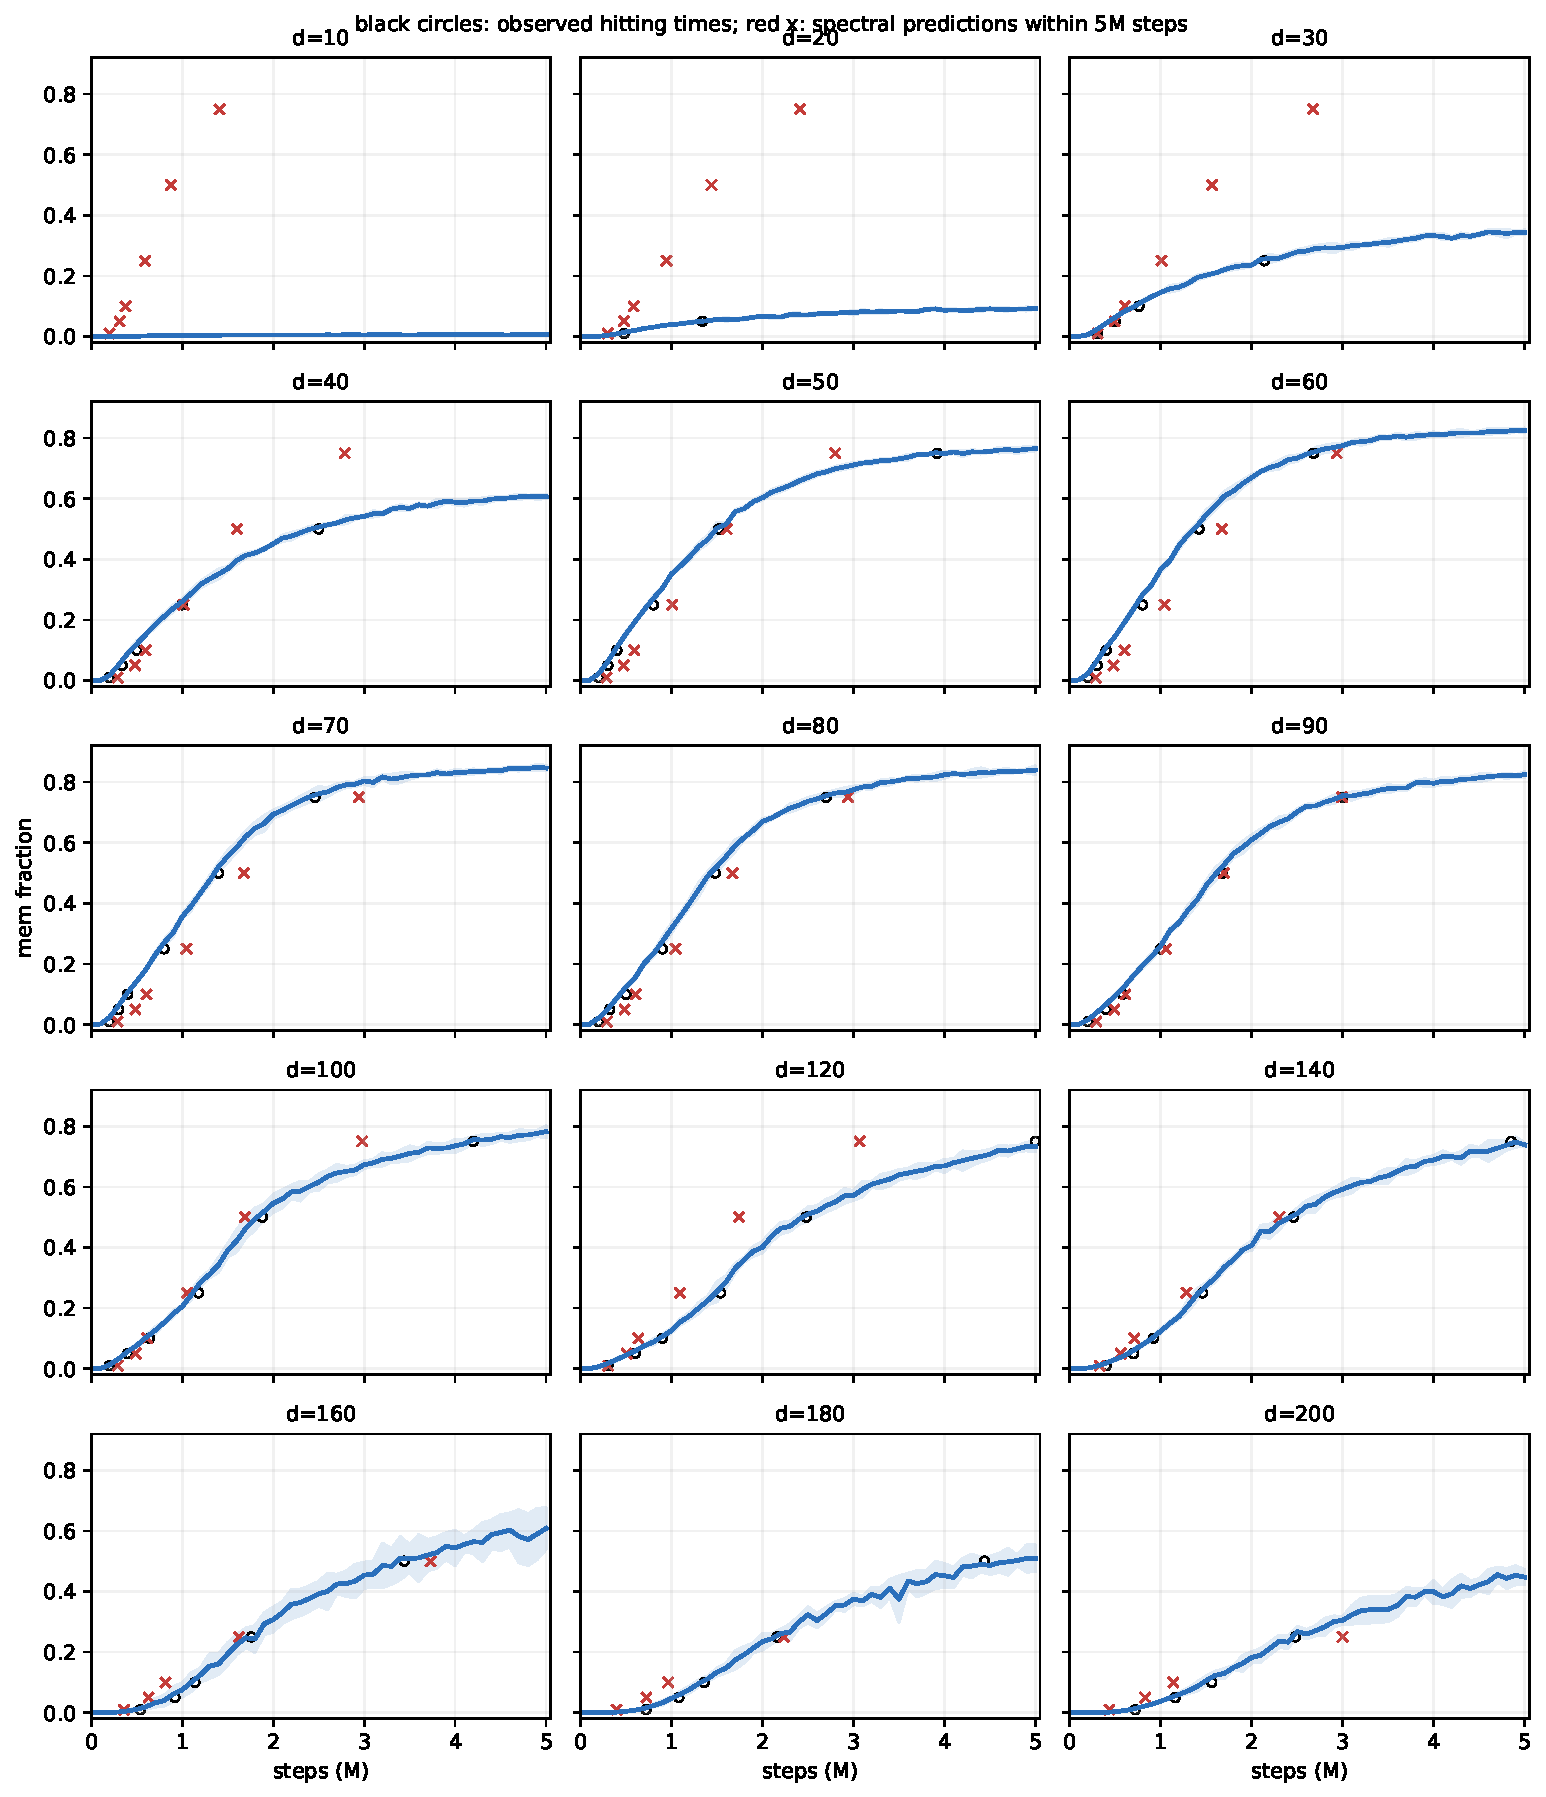
\includegraphics[width=\linewidth]{figures/celeba_spectral_mem_small_multiples.pdf}
    \caption{CelebA.}
  \end{subfigure}\hfill
  \begin{subfigure}{0.49\textwidth}
    \centering
    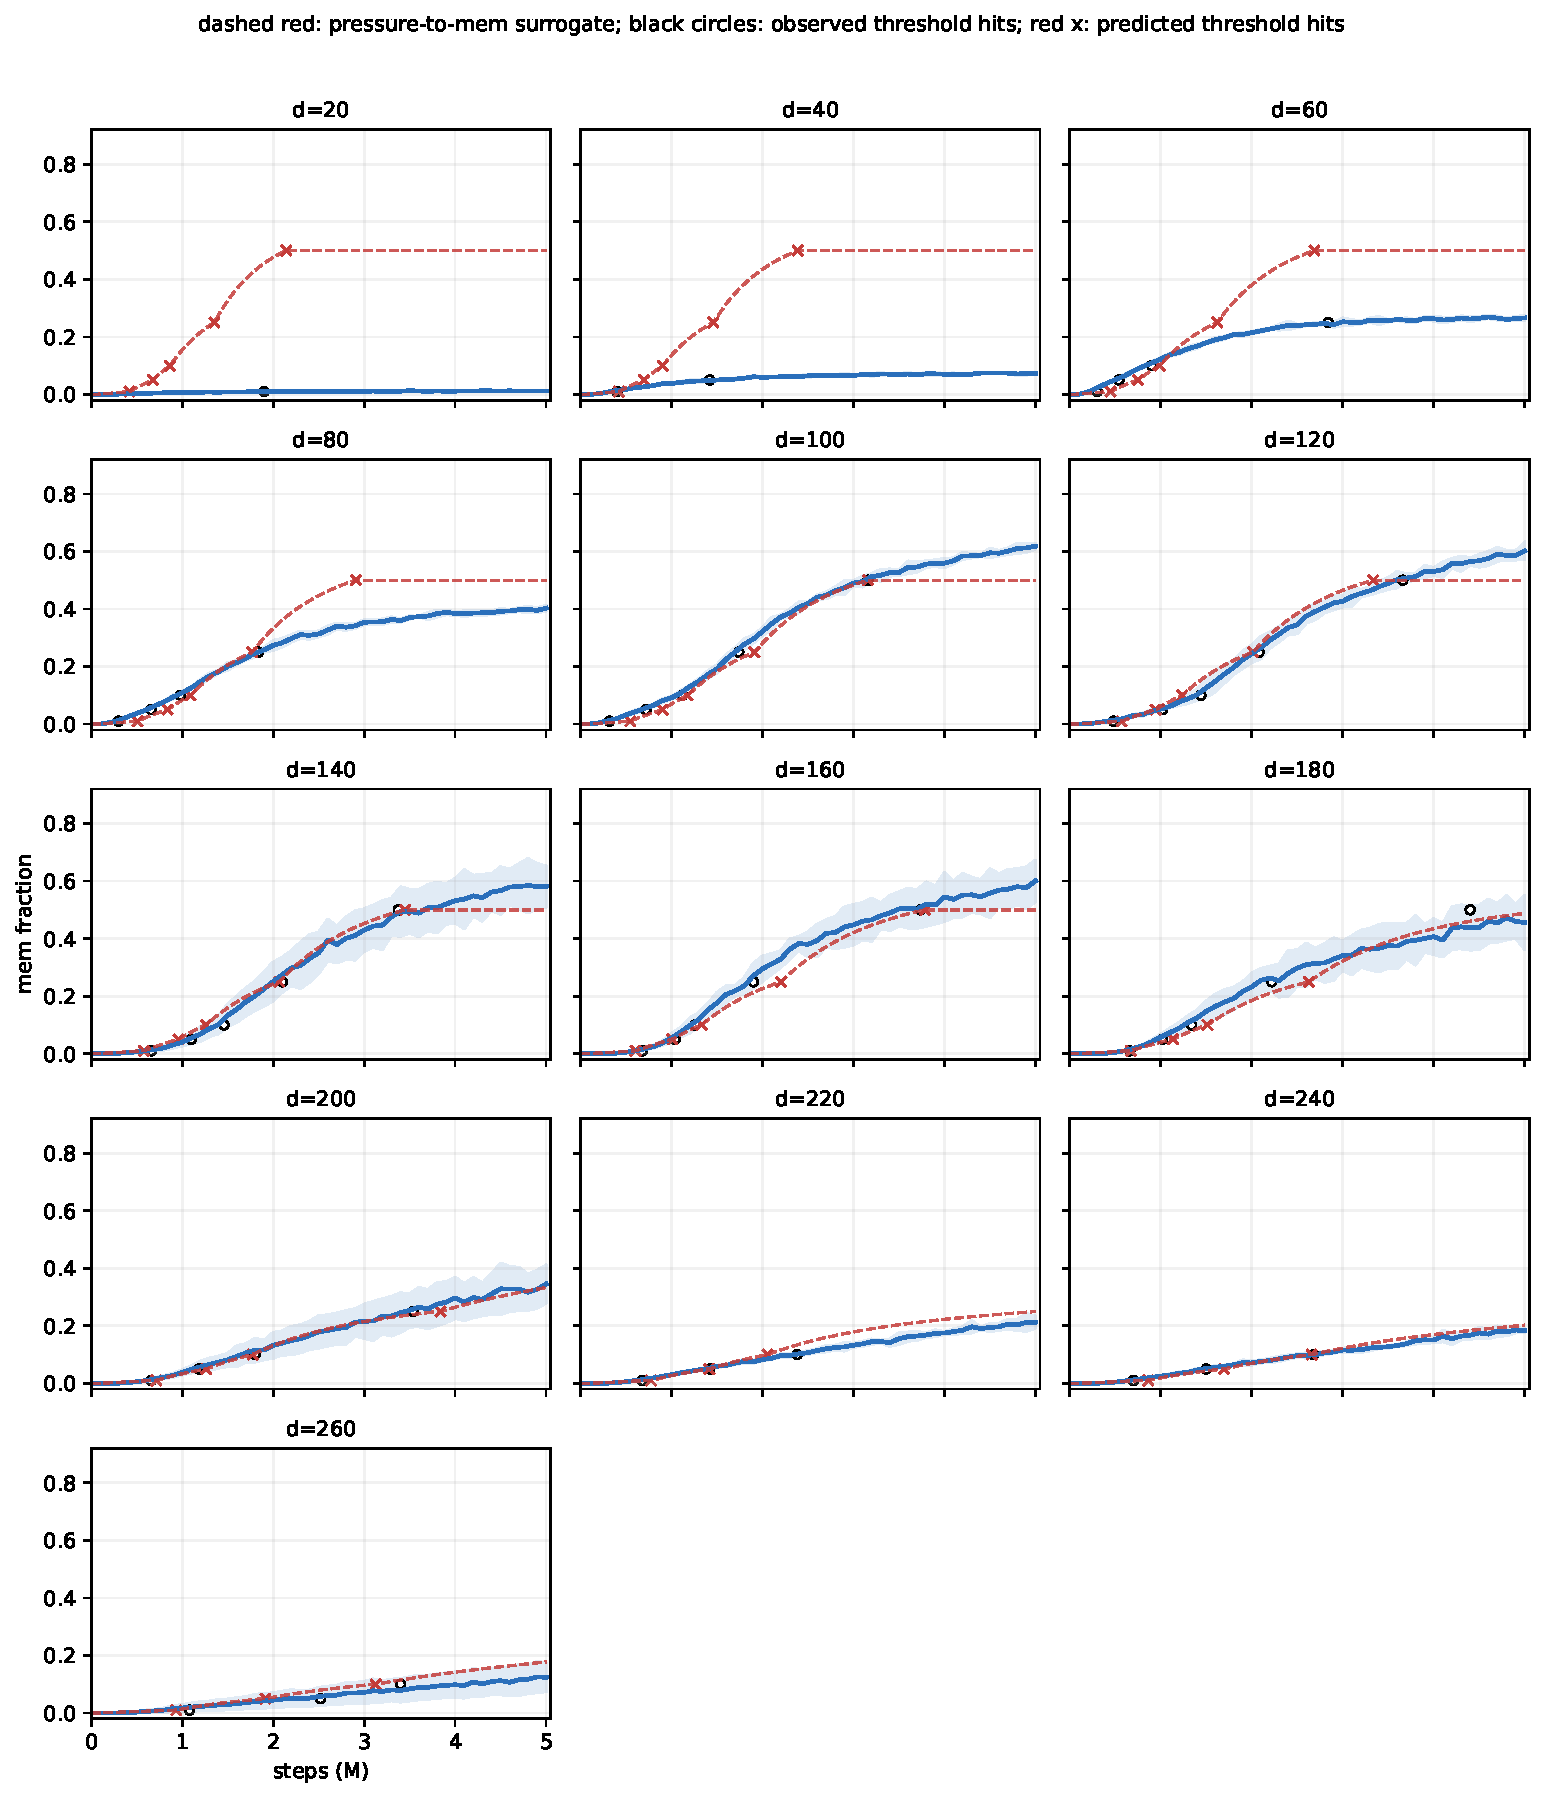
\includegraphics[width=\linewidth]{figures/cifar10_spectral_mem_small_multiples.pdf}
    \caption{CIFAR-10.}
  \end{subfigure}
  \caption{\textbf{Spectral memorization predictor.} Empirical
    memorization curves with predicted iso-memorization checkpoints
    overlaid. The calibration is global across dimensions within a
    dataset; no per-$d$ fit is used. The strongest match is the
    ordering and onset pattern across latent widths, which is the
    quantity needed for a stopping-time heuristic.}
  \label{fig:real-spectral-predictor}
\end{figure*}
